\documentclass{article}
\usepackage{tikz}
\usetikzlibrary{intersections}

\begin{document}

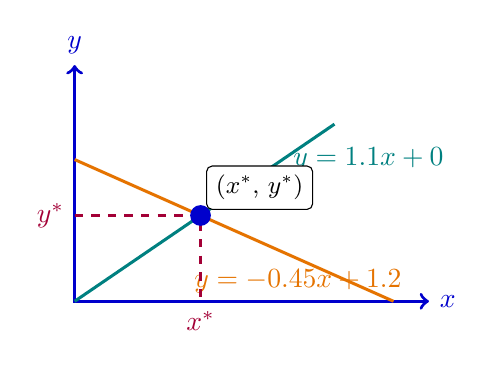
\begin{tikzpicture}[scale=1.5]
    % Draw axes
    \draw [<->,line width=1.2pt,blue!80!black] (0,2) node (yaxis) [above] {\textbf{$y$}}
        |- (3,0) node (xaxis) [right] {\textbf{$x$}};
    % Draw two intersecting math lines
    \draw[teal, line width=1.1pt] (0,0) coordinate (l_1) -- (2.2,1.5) coordinate (l_2) node[pos=0.8,right] {$y=1.1x+0$};
    \draw[orange!90!black, line width=1.1pt] (0,1.2) coordinate (m_1) -- (2.7,0) coordinate (m_2) node[pos=0.7,below] {$y=-0.45x+1.2$};
    % Calculate the intersection of the lines l_1 -- l_2 and m_1 -- m_2
    \coordinate (inter) at (intersection of l_1--l_2 and m_1--m_2);
    % Draw lines indicating intersection with y and x axis
    \draw[dashed, purple!85!black, line width=0.9pt] (yaxis |- inter) node[left] {$y^{*}$}
        -| (xaxis -| inter) node[below] {$x^{*}$};
    % Draw a dot to indicate intersection point
    \fill[blue!80!black] (inter) circle (2.5pt);
    % Add intersection node label
    \node[draw=black, fill=white, rounded corners=2pt, font=\small, above right=2pt] at (inter) {$(x^{*},\,y^{*})$};
\end{tikzpicture}
\end{document}